\section{问题重述}
\subsection{问题背景}

微网通过协调分布式电源、储能与用户负载，实现局部供需平衡，并可与外部电网协同运行\upcite{nea2024microgrid}。我国2021年源网荷储指导意见提出，依托光伏和并网型微电网推进园区、居民区能源协同利用\upcite{ndrc2021integration}。然而，光伏等新能源的间歇性与波动性，增加了供需平衡与运行调度的难度\upcite{nea2023bluebook}。\par

储能协同优化运行可增强系统调峰能力，促进新能源消纳\upcite{ndrc2021storage}。在本题中，微网需在容量、功率和效率约束下，协调计划购电与储能充放电，并应对预测偏差、日内调整费用及电价波动。因此，需要研究不同信息条件下的购电策略，在满足负载需求的同时控制总购电费用。

\subsection{问题要求}

根据题目所给的电价、负载、光伏发电及预报数据，在满足负载需求和储能设备运行约束的前提下，以尽可能降低购电费用为目标，建立数学模型研究以下四个问题：

\textbf{问题一：}在每天的电价和小区负载相同、已知一天光伏发电功率预测数据的条件下，建立每天0:00制定当天计划购电策略的数学模型，保证供电不低于负载，且储能设备在0:00与24:00的储电量相同。利用附件1和附录1的数据，给出计划购电量、购电费用及储能充放电安排，并按要求展示指定时段及全天结果。

\textbf{问题二：}在每天的电价相同、负载与光伏出力随时间变化的条件下，利用附件1中的电价及附件2的数据，在每天0:00制定当天计划购电策略。供电缺口通过紧急购电补足，其单价为交易时刻电价的5倍，其余购电费用按计划购电量计算。给出购电与储能运行结果，并统计紧急购电的时段和电量。

\textbf{问题三：}利用每天0:00、6:00、12:00和18:00发布的未来24小时整点光伏预报，建立包含初始购电计划与日内调整的调控模型。减购部分按交易时刻电价的50\%计算违约费用，增购部分按其1.5倍计价，综合考虑计划购电、紧急购电和调整相关费用。给出相应购电与储能运行结果，并分析是否需要引入其他时刻的预报调整购电策略。

\textbf{问题四：}将外网电价扩展为实时波动情形，结合附件2中的负载与光伏实际数据、附件3中的光伏预报及附件4中的电价数据，重新建立并求解问题二和问题三对应的购电策略模型，给出波动电价下的购电费用、购电安排、储能充放电及紧急购电结果。

\Needspace{0.45\textheight}
\subsection{我们的工作}

本文围绕四问开展建模、求解与检验，总体流程如图\ref{fig:overall-workflow}所示。

\begin{figure}[H]
    \centering
    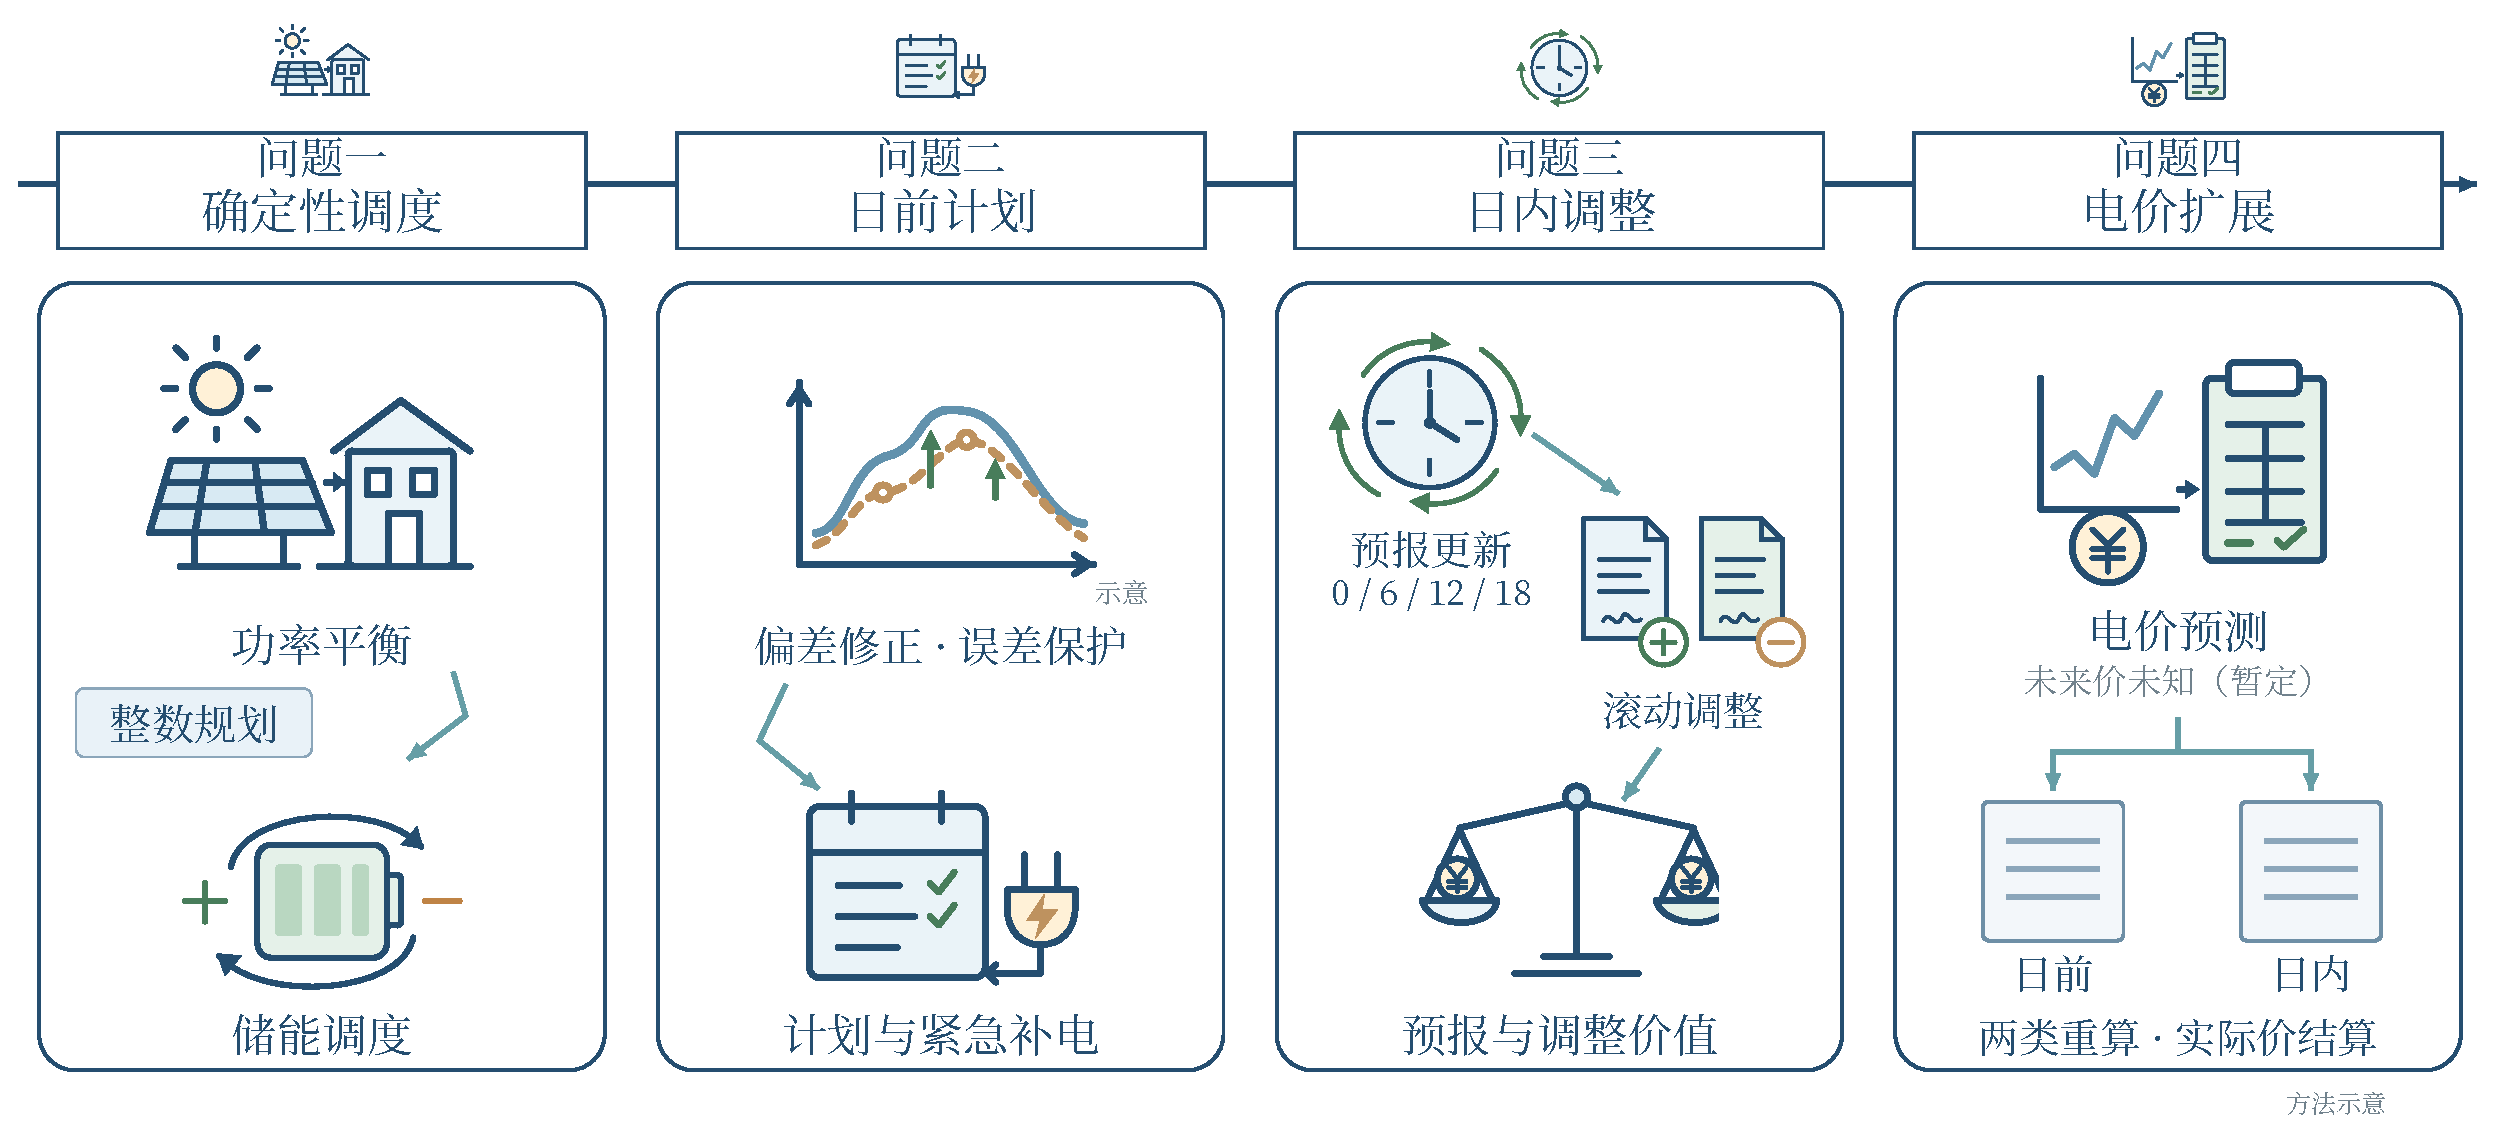
\includegraphics[width=\textwidth]{figures/总体流程图_图示版.pdf}
    \caption{本文总体研究流程}
    \label{fig:overall-workflow}
\end{figure}
